\documentclass{beamer}
\usepackage{listings}
\usepackage{lmodern}

\lstset{language=C,
    basicstyle=\ttfamily,
    keywordstyle=\bfseries,
    showstringspaces=false,
    morekeywords={scan, in, forall, shift, to, def, downto, is, endif, endfor, enddef, upto, and, or}
}


\usetheme{metropolis}

\title{Li, Li, Huo - Optimal In-Place Suffix Sorting}
\date{\today}
\author{Patrick Indri}
\institute{DSSC - Algorithmic Design Exam}

\setlength{\textfloatsep}{2.0pt plus 1.0pt minus 2.0pt}


\begin{document}
  \maketitle

  \begin{frame}{Index}
    \begin{itemize}
      \item Problem setting;
      \item Naive solution;
      \item Preliminary notions;
      \item Suffix sorting for read-only integer alphabets;
      \item Additional results and conclusions;
      \item Auxiliary material.
    \end{itemize}
  \end{frame}

  \begin{frame}{Problem Setting}
    \textit{Suffix Arrays}: a space-saving alternative to suffix trees.
    \begin{block}{Definition}
      \vspace{1pt}
      Given a string $T = T[0, \dots, n-1]$ where each $T[i] \in \Sigma$ integer alphabet, the \textit{suffix array} $SA$ contains the indices of all suffixes of $T$ which are sorted in lexicographical order.
    \end{block}
    \pause
    \begin{block}{Example}
      \vspace{1pt}
      $T = "1120"$, the suffixes are $\{ 1120, 220, 20, 0 \}$. Since $suf(3)<suf(0)<suf(2)<suf(1)$, then $SA = [3021]$.
    \end{block}
  \end{frame}

  \begin{frame}{Problem Setting}
    \begin{block}{Problem}
      \vspace{1pt}
      Construct $SA$ for a given string $T$.
    \end{block}
    \begin{block}{Main Theorem}
      \vspace{1pt}
      There is an in-place linear time algorithm for suffix sorting over integer alphabets, even if the input string $T$ is read only and the size of the alphabet $|\Sigma|$ is $O(n)$.
    \end{block}
  \end{frame}


  \begin{frame}{Naive Solution}
    \begin{itemize}
      \item Get all the suffixes and sort them using \textit{Quicksort}, while retaining their original indices. $O(n\log n)$ comparisons for sorting, $O(n)$ to compare suffixes: worst case is $O(n^2\log n)$.
      \item Build a suffix tree in $O(n)$ and perform a depth-first traversal on it in $O(n)$.    \end{itemize}
  \end{frame}

  \begin{frame}{Preliminary Notions}
    \textbf{Notations:}
    \begin{itemize}
      \item $suf(i)$ is said to be $S$-suffix if $suf(i) < suf(i+1)$. Otherwise, it is $L$-suffix;
      \item $suf(i)$ is said to be $LMS$-suffix if $suf(i)$ is $S$-suffix and $suf(i-1)$ is $L$-suffix;
    \end{itemize}

    \begin{block}{Note}
      \vspace{1pt}
      Types ($S$ or $L$, and $LMS$) can be computed by a linear scan of $T$.
    \end{block}

    \pause

    \begin{block}{Example: $T = "3122120"$}
      \vspace{-5pt}
      \begin{center}
        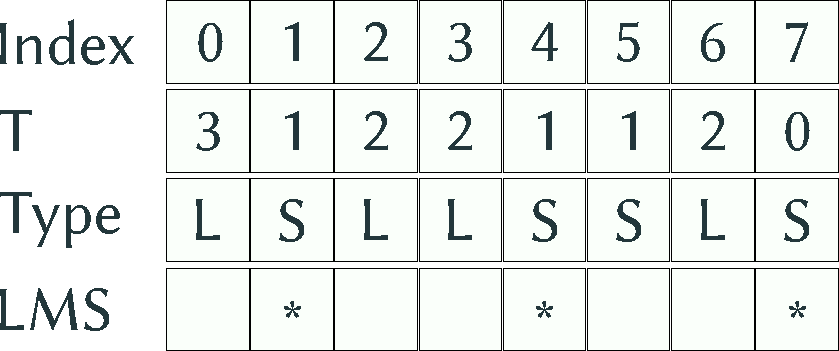
\includegraphics[width=0.5\textwidth]{img/preliminary.pdf}
      \end{center}
    \end{block}
  \end{frame}



  \begin{frame}{Suffix Sorting for Read-only Integer Alphabets}
    \textbf{Definitions and assumptions:}
    \begin{itemize}
      \item $n_S$ ($n_L$) denotes the number of $S$-suffixes ($L$-suffixes);
      \item $n_L \le n_S$;
      \item $n_1$ denotes the number of $LMS$-suffixes;
      \item $SA[0, \dots, n-1]$ will store the result;
      \item Bucket: set of suffixes with the same first character.

    \end{itemize}
    \pause

    \textbf{Algorithm:}
    \begin{enumerate}
      \item Sort all $LMS$-characters of $T$;
      \item Induced sort all $LMS$-substrings from sorted $LMS$-characters;
      \item Construct the reduced problem $T_1$ from sorted $LMS$-substrings;
      \item Sort the $LMS$-suffixes by recursively solving $T_1$;
      \item Induced sort all suffixes of $T$ from the sorted $LMS$-suffixes.
    \end{enumerate}
  \end{frame}


  \begin{frame}{1. Sort all $LMS$-characters of $T$}\label{1}
    The $LMS$-characters can be sorted with \textit{Counting Sort}, using $SA[0, \dots, n/2]$ as the counting array and storing the result in $SA[n-n_1, \dots, n-1]$.
\hyperlink{AUX1}{\beamerbutton{AUX}}
    \begin{figure}
    \centering
    \begin{minipage}{.5\textwidth}
      \centering
      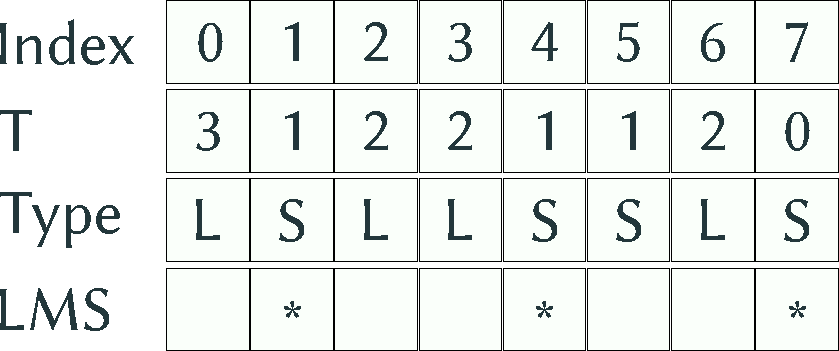
\includegraphics[width=.9\linewidth]{img/preliminary.pdf}
    \end{minipage}%
    \begin{minipage}{.5\textwidth}
      \centering
      
\includegraphics[width=.9\linewidth]{img/SA_1.pdf}
    \end{minipage}
    \end{figure}

    The sorting step takes $O(n)$ time and uses $O(1)$ workspace.

  \end{frame}


  \begin{frame}{2. Induced sort all $LMS$-substrings from sorted $LMS$-characters}
    This step is analogous to step 5.

    After this step, indices of the ordered $LMS$-substrings are stored in $SA[n-n_1, \dots, n-1]$.

    \begin{figure}
    \centering
    \begin{minipage}{.5\textwidth}
      \centering
      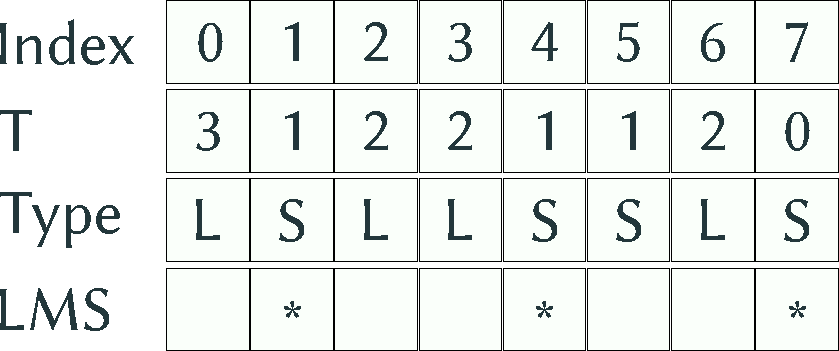
\includegraphics[width=.9\linewidth]{img/preliminary.pdf}
    \end{minipage}%
    \begin{minipage}{.5\textwidth}
      \centering
      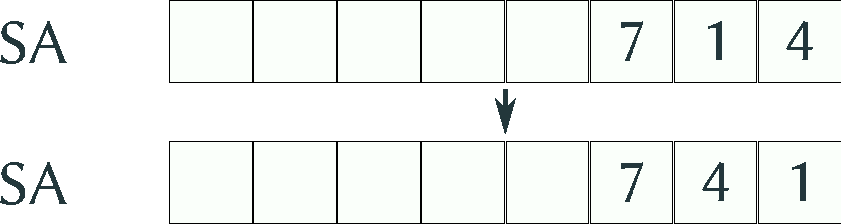
\includegraphics[width=.9\linewidth]{img/SA_2.pdf}
    \end{minipage}
    \end{figure}

    $LMS$-substrings are $\{ 1121, 1120, 0 \}$.
  \end{frame}

  \begin{frame}{3. Construct the reduced problem $T_1$}
    Using the lexicographical order of the $LMS$-substrings, build the reduced problem $T_1$ and store it in $T[0, \dots, n_1]$.
$T_1$ can be obtained by a liner scan of $SA$, thus using $O(n)$ time and $O(1)$ workspace.

    \begin{figure}
    \centering
    \begin{minipage}{.5\textwidth}
      \centering
      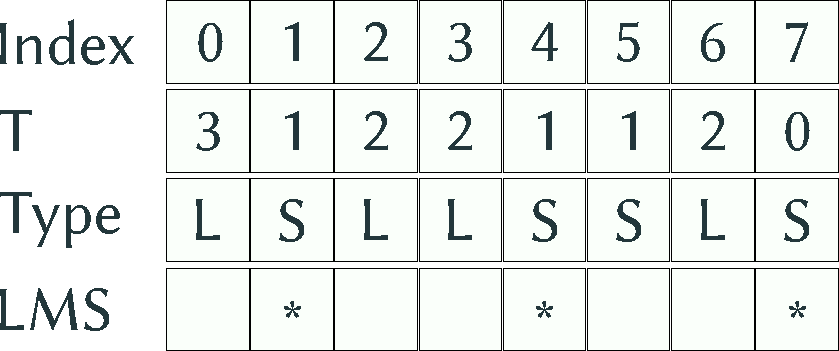
\includegraphics[width=.9\linewidth]{img/preliminary.pdf}
    \end{minipage}%
    \begin{minipage}{.5\textwidth}
      \centering
      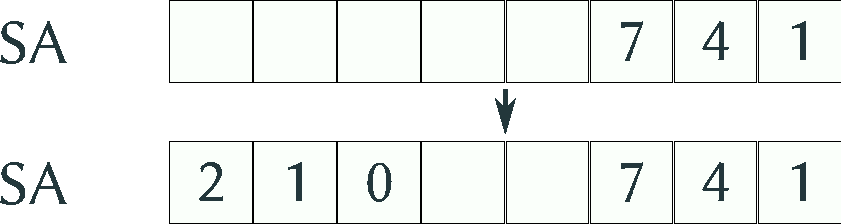
\includegraphics[width=.9\linewidth]{img/SA_3.pdf}
    \end{minipage}
    \end{figure}

    $LMS$-substrings are $\{ 1121, 1120, 0 \}$.

  \end{frame}


  \begin{frame}{4. Sort the $LMS$-suffixes by recursively solving $T_1$}
    $T_1$ can be solved iteratively in linear time\footnote{$\mathcal{T}(n) = \mathcal{T}(n/2) + n = n(1 + 1/2 + 1/4 + 1/8 + \dots + 1/\log_2 n ) \in \Theta(n)$} with no additional workspace. It is stored at the beginning of $SA$. The $LMS$-suffixes are sorted using linear scans and the solution of $T_1$.

    \begin{figure}
      \centering
      \begin{minipage}{.5\textwidth}
        \centering
        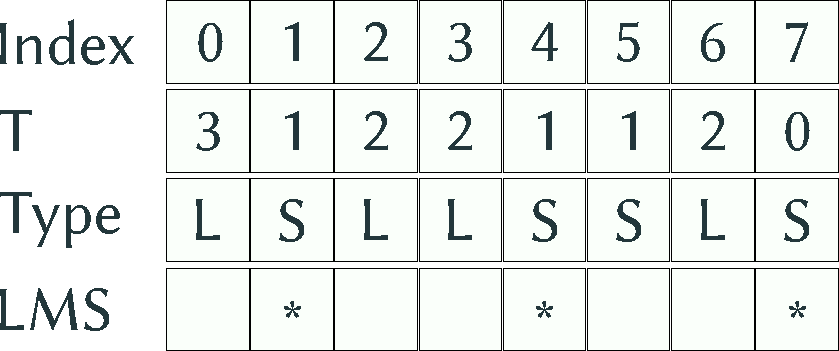
\includegraphics[width=.9\linewidth]{img/preliminary.pdf}
      \end{minipage}%
      \begin{minipage}{.5\textwidth}
        \centering
        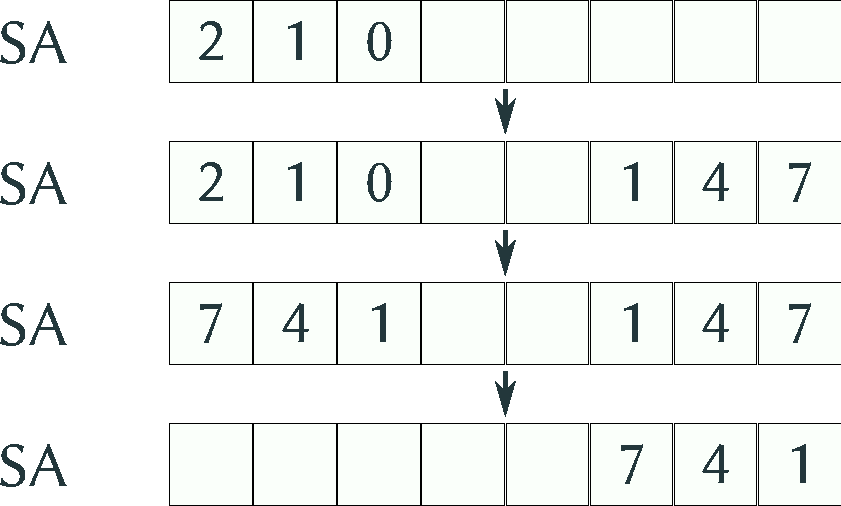
\includegraphics[width=.9\linewidth]{img/SA_4.pdf}
      \end{minipage}
    \end{figure}

    $LMS$-suffixes are $\{ 1221120, 1120, 0 \}$.

    The complexity of this step is $O(n)$ in time and $O(1)$ in workspace.
    \vspace{1pt}

  \end{frame}


  \begin{frame}{5. Induced sort all suffixes of $T$ from the sorted $LMS$-suffixes}
    It can be demonstrated that sorting the $n_L$ $L$-suffixes from the sorted $LMS$-suffixes is symmetrical as sorting the $n_S$ $S$-suffixes from the sorted $L$-suffixes. Suppose $L$-suffixes are sorted.

    \begin{figure}
      \centering
      \begin{minipage}{.5\textwidth}
        \centering
        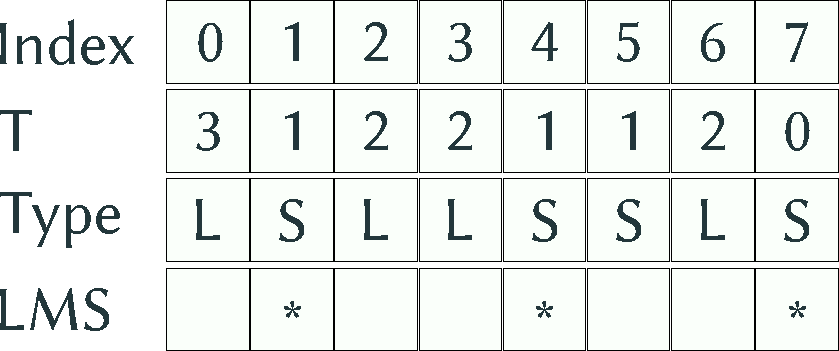
\includegraphics[width=.9\linewidth]{img/preliminary.pdf}
      \end{minipage}%
      \begin{minipage}{.5\textwidth}
        \centering
        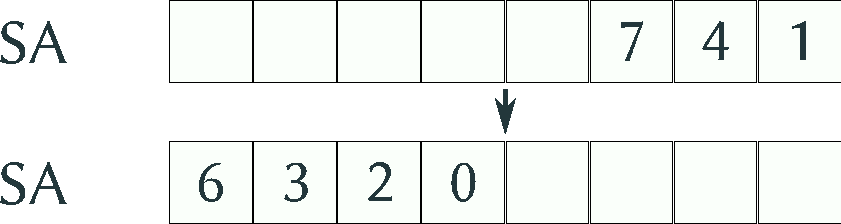
\includegraphics[width=.9\linewidth]{img/SA_5.pdf}
      \end{minipage}
    \end{figure}

    $L$-suffixes are $\{ 31221120, 221120, 21120, 20 \}$.

  \end{frame}


  \begin{frame}{5. Induced sort all suffixes of $T$ from the sorted $LMS$-suffixes}\label{5}
    \begin{block}{Pointer Data Structure}
      \vspace{1pt}
      Built in linear time, indicates the bucket tails of a $S$-suffix in constant time. Occupies at most $c_P = cn/\log n$ words, placed at the end of $SA$. \hyperlink{AUX5.pointer}{\beamerbutton{AUX}}
    \end{block}
    \begin{block}{Interior Counter Trick}
      \vspace{1pt}
      Dynamically maintain the $RF$-pointers (rightmost free pointers) for each bucket. \hyperlink{AUX5.counter}{\beamerbutton{AUX}}
    \end{block}
    \pause
    The ordering of the $S$-suffixes proceeds in two steps:
    \begin{enumerate}
      \item Construct a \textit{pointer data structure} $\mathcal{P}$ and, combining it with the \textit{interior counter trick} induce the first $n_S - c_P$ $S$-suffixes;
      \item Use \textit{Binary Search} and the \textit{Interior Counter Trick} on the last $c_P$ $S$-suffixes.
    \end{enumerate}
  \end{frame}


  \begin{frame}[fragile]{5. Induced Sort Algorithm}
    Suppose $L$-indices are already sorted in their buckets.
    \begin{lstlisting}
def InducedSort(T, SA):
  for i = nL downto 0:
    j = SA[i] - 1 # Indicizes the bucket.
    if T[j] is S-type:
      *RF[j] = j
      RF[j] = next_free_entry
    endif
  endfor
enddef
    \end{lstlisting}

    For each query of $RF$, the tail of the bucket is provided in constant time by the pointer data structure, from that the interior counter trick indicates the $RF$ entry.
  \end{frame}

  \begin{frame}{5. Induced sort all suffixes of $T$ from the sorted $LMS$-suffixes}
    The first $n_S - c_P$ $S$-suffixes can be ordered in linear time with no additional workspace. The remaining suffixes can be sorted analogously, using binary search to find the tails of the buckets, since $c_P \log n = O(n)$ and time linearity is preserved.

    A stable, in place linear time merging can be used to merge the sorted $S$- and $L$-suffixes.
    \begin{center}
      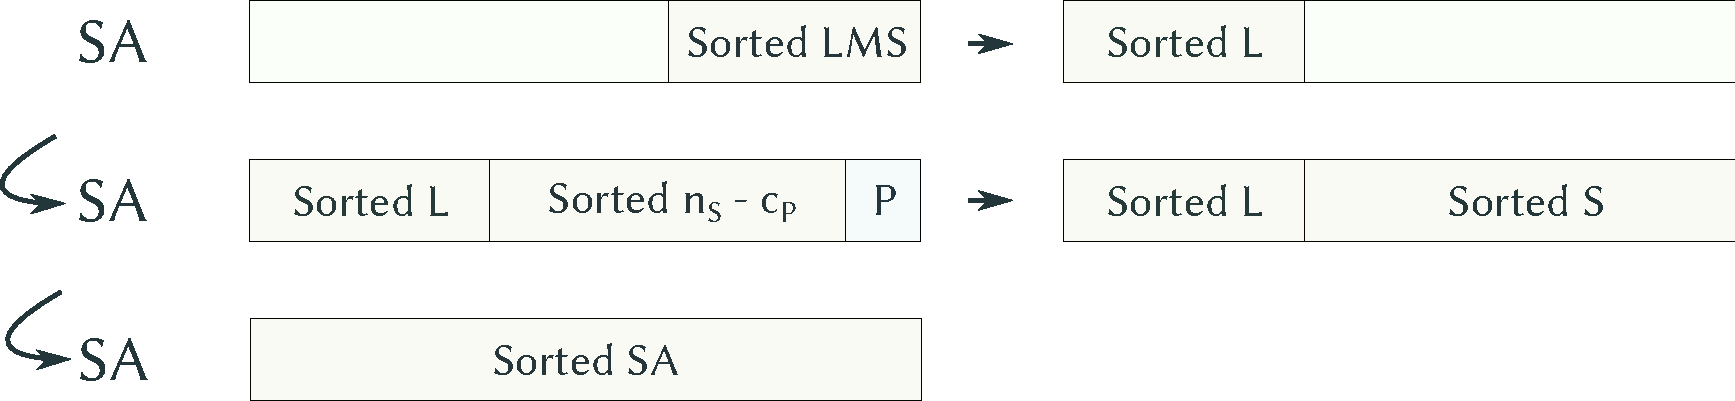
\includegraphics[width=1\textwidth]{img/SA_sorted.pdf}
    \end{center}
  \end{frame}


  \begin{frame}{Additional results and conclusion}
    \begin{block}{(Read-only) Integer Alphabets}
      \vspace{1pt}
      Considering all the steps, it follows that the algorithm takes $O(n)$ time and $O(1)$ workspace to compute the suffix array of a string $T$ over integer alphabets $\Sigma$, where $T$ is read-only and $|\Sigma| = O(n)$.
    \end{block}

    The result trivially holds for non-read-only integer alphabets.

    \pause

    \begin{block}{Read Only General Alphabets}
      \vspace{1pt}
      For read-only general alphabets (i.e., only comparisons allowed on $T$) there is an in-place $O(n\log n)$ time algorithm for suffix sorting.
    \end{block}

    \pause

    \begin{block}{References}
      \vspace{1pt}
      Li, Zhize, Jian Li, and Hongwei Huo. "Optimal in-place suffix sorting." \textit{International Symposium on String Processing and Information Retrieval}. Springer, Cham, 2018.
    \end{block}

  \end{frame}

  \section{Auxiliary Material}
  \begin{frame}{AUX: Sort all $LMS$-characters of $T$}\label{AUX1}
    Since $|\Sigma| = O(n)$, assume $\exists d \in \mathbb{N}$ s.t. $|\Sigma| \le dn$. Divide $LMS$-characters in $2d$ partitions, where partition $i$ contains elements in $\left[ \frac{i|\Sigma|}{2d} +1, \frac{(i+1)|\Sigma|}{2d} \right]$. Since

    $$\frac{|\Sigma|}{2d} \le \frac{dn}{2d} = \frac{n}{2},$$

    $SA[0, \dots, n/2]$ can be used as a counting array. \hyperlink{1}{\beamerbutton{$\hookleftarrow$}}
  \end{frame}

  \begin{frame}[fragile]{AUX: Interior counter trick - 1}\label{AUX5.counter}
    Consider a bucket of size $m$, indexing it as $SA_S \{0, \dots, m-1 \}$. Define the special symbols $B_H$, $B_T$, $E$, $R_1$ and $R_2$. \texttt{Index(i)} denotes the index of the $i$-th $S$-suffix of the bucket. The position of the tail, i.e., \texttt{m-1}, is given by the pointer data structure.
    \begin{lstlisting}
def InteriorCounterTrick(SAs):
  SAs[0]=BH, SAs[m-2]=E, SAs[m-1]=BT
  # O(m) time.
  if SAs[m-1]=BT and
    (SAs[m-2]=E or SAs[m-SAs[m-2]-3]!=BH):
    for i=1 upto m-3:
      SAs[m-2-i]=Index(i)
      SAs[m-2]++   # Acts as a counter.
    endfor
  endif
    \end{lstlisting}
  \end{frame}

  \begin{frame}[fragile]{AUX: Interior counter trick - 2}
    \begin{lstlisting}
  # O(m) time.
  if SAs[m-1]=BT and SAs[m-SAs[m-2]-3]=BH:
    shift SAs[1,...,m-3] to SAs[2,...m-2]
    SAs[1]=Index(m-2)
    SAs[m-1]=R2
  endif
  # O(m) time.
  if SAs[m-1]=R2;
    shift SAs[1,...,m-2] to SAs[2,...,m-1]
    SAs[1]=Index(m-1)
    SAs[0]=R1
  endif
    \end{lstlisting}
  \end{frame}

  \begin{frame}[fragile]{AUX: Interior counter trick - 3}

    \begin{lstlisting}
  # O(m) time, need to scan from tail
  # backwards to find R1.
  else:
    SAs[0]=Index(m)
enddef
    \end{lstlisting}

    The function consists of four steps, each $O(m)$ time, assuming that the tail of a bucket is known. It uses $O(1)$ workspace and, for all the buckets, results in $O(n)$ time. \hyperlink{5}{\beamerbutton{$\hookleftarrow$}}

  \end{frame}


  \begin{frame}[fragile]{AUX: Pointer data structure - 1}\label{AUX5.pointer}
    Assuming $|\Sigma| \le dn$, divide the $S$-suffixes of $T$ in $4d$ parts, according to their first character. Let $D_i$ denote the pointer data structure of the $i$-th part. $D_0$ can be constructed as follows (analogously for the others). For brevity, $\texttt{b} = |\Sigma|/4d$.

    \begin{lstlisting}
def PointerDataStructure(T, SAs):
  SAs[i]=1 forall i in [1,b]
  for i=n-1 downto 0:
    if T[i] is S-type and in [1,b]: SAs[T[i]]++
  endfor
    \end{lstlisting}

  \end{frame}

  \begin{frame}[fragile]{AUX: Pointer data structure - 2}
    \begin{lstlisting}
  sum=-1
  for i=1 upto b:
    sum+=SAs[i]
    SAs[i]=sum
  endfor
enddef
    \end{lstlisting}

    For every $S$-suffix for which $T[i]\in SA_S[i,|\Sigma|/4d]$, $SA_S[T[i]] - T[i]$ indicates the tail of the bucket $T[i]$: the tail of a bucket can be obtained in constant time. \hyperlink{5}{\beamerbutton{$\hookleftarrow$}}

  \end{frame}



\end{document}
